\documentclass[journal]{IEEEtran}
\usepackage{amsmath,amssymb}
\usepackage{booktabs}
\usepackage{graphicx}
\usepackage{hyperref}
\usepackage{multirow}
\usepackage{xcolor}

% ---- Revision markup: \markuptrue shows changes (blue = new or changed text,
% red bracketed = removed claim); \markupfalse typesets the clean revision. ----
\newcommand{\PENDING}[1]{\textbf{\color{red}[PENDING: #1]}}
\newif\ifmarkup
\markuptrue
\ifmarkup
\newcommand{\added}[1]{{\color{blue}#1}}
\newcommand{\removed}[1]{{\color{red}[\textit{Removed:} #1]}}
\else
\newcommand{\added}[1]{#1}
\newcommand{\removed}[1]{}
\fi

% ---- Anonymization toggle: \anonymoustrue for review submission, \anonymousfalse for camera-ready ----
\newif\ifanonymous
\anonymoustrue

\ifanonymous
\newcommand{\repourl}{\url{https://anonymous.4open.science/status/moba-draft-policies}}
% Anonymized review mirror of the deployed web tool (single line to update):
\newcommand{\deployurl}{\url{https://draft-assistant-review.vercel.app}}
\else
\newcommand{\repourl}{\url{https://github.com/maxsegan/moba-draft-policies}}
\newcommand{\deployurl}{\url{https://www.hotsfever.com}}
\fi
% -----------------------------------------------------------------------------------------------------

\begin{document}

\title{Diagnosing and Repairing Out-of-Distribution\\ Failure in MOBA Draft Policies}
\ifanonymous
\author{Anonymous Authors}
\else
\author{Max~Segan, Ernest~Pysher, James~Frankel, and Hod~Lipson}
\fi
\maketitle

\begin{abstract}
In multiplayer online battle arena (MOBA) drafting, two teams alternately ban and pick heroes from a shared pool to build competing five-hero compositions, and a noisy match decides the winner. In Heroes of the Storm, a 90-hero pool spans $7.2 \times 10^{14}$ matchups; \added{1.95 million} ranked drafts cover a vanishing, clustered fraction, so out-of-distribution behavior dominates policy quality. Search exploits learned value functions' out-of-distribution optimism, assembling structurally broken teams rated as competitive, and pessimistic offline reinforcement learning does not repair this: conservative and implicit Q-learning collapse to behavioral cloning, and mildly conservative Q-learning to a near-deterministic ten-hero policy. We decompose draft-policy quality into composition safety and interaction-awareness, with metrics that detect both collapses. \added{We also report a pitfall in our own first pipeline: value-function features built from aggregate statistics that contained each game's own outcome made the value function overconfident and let search chase its errors. With out-of-fold statistics and judges that share no data with any agent, domain features, synthetic data for never-observed compositions, and Monte Carlo tree search yield agents that are safe and interaction-aware, and a structural constraint mask guarantees validity at no measured cost. Deep search beats every behavior-anchored method under all six independent judges (0.60 vs.\ 0.44 tournament win probability), while its gains from extra simulations and from domain features are smaller than the agents' own value function suggests.} Code, models, and the in-browser agent are open-source.
\end{abstract}

\begin{IEEEkeywords}
MOBA drafting, team assembly, offline reinforcement learning, Monte Carlo tree search, out-of-distribution generalization.
\end{IEEEkeywords}

\section{Introduction}


Drafting has a structure with three properties that drive everything in this paper: a small number of opponents (here, two) alternately claim discrete, rivalrous elements from a shared pool to assemble competing sets; the value of a set depends nonlinearly on interactions within it and against the opposing set, not only on element quality; and the winner is determined by a noisy downstream process rather than by rule. The same structure recurs wherever rivals assemble from a shared scarce pool (sports drafts, roster auctions, deck drafting, procurement), but those instances lack instrumentation; drafting in multiplayer online battle arena (MOBA) games offers millions of logged episodes under fixed rules, a natural model organism. In Heroes of the Storm (HotS), two teams of five alternate through 16 actions, banning 6 heroes and picking 10 from a pool of 90, before the match itself is played. We study HotS because it is in maintenance mode: a fixed 90-hero pool across 4.5 years of one major version yields an unusually clean stationary corpus. The draft matters: models that observe only the completed draft predict match outcomes at \added{about 57\%} accuracy \added{on held-out games}, a large edge in a balanced competitive game.

Two properties of the domain make learned drafting hard. The first is coverage. A 90-hero pool admits roughly $7.2 \times 10^{14}$ distinct final matchups ($\tfrac{1}{2}\binom{90}{5}\binom{85}{5}$), and our corpus of \added{1.95 million} ranked drafts covers a vanishing fraction of that space, and not uniformly: human play clusters around popular heroes and familiar groupings, \added{leaving the rest empty}. Any drafting policy must therefore behave sensibly in states it has effectively never observed. The second is evaluation: unlike chess or Go, where the terminal state determines the winner by rule, a completed draft only shifts the odds of the match that follows, so the reward signal for training and search is itself a win probability model estimated from the same sparse, clustered data, and value and policy errors compound.

\begin{figure}[t]
\centering
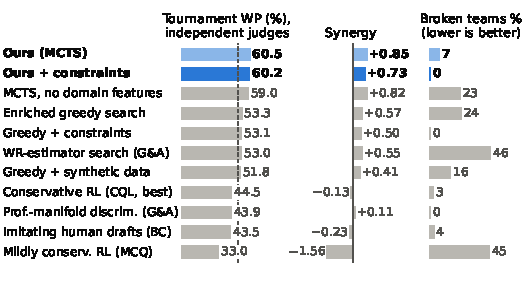
\includegraphics[width=\columnwidth,height=1.95in,keepaspectratio]{fig_glance_revision.pdf}
\caption{Results at a glance: the \added{twelve}-strategy round-robin (\added{132} ordered pairs $\times$ 200 drafts; Section~\ref{sec:tournament}). First column: \added{mean win probability under four judges that share no data with any agent} (dashed line: 50\%); the CQL row shows the better variant per column. Anchoring to human behavior is safe but interaction-blind; unstructured value search is interaction-aware but unsafe; \added{MCTS over a value function reaches both, and constraint masking (Section~\ref{sec:constrained}) removes its residual broken teams at no cost in win probability.}}
\label{fig:glance}
\end{figure}
Prior work has treated draft outcome prediction and hero recommendation largely as supervised learning problems and reports respectable held-out accuracy~\cite{chen2018drafting,gourdeau2021discriminative,summerville2016draft,lee2022draftrec}. We show that this accuracy is a misleading foundation for a drafting policy. Three value functions \added{within 0.2 percentage points of held-out accuracy (57.6--57.7\%)} yield greedy policies that disagree on roughly 90\% of decisions. When used for search, each model's out-of-distribution behavior, not its accuracy, determines policy quality: the optimizer seeks out states vanishingly rare in human play, a team of five tanks, or one with no healer, and the models score them as competitive. The evidence that such teams fail exists, but not in any individual game: lineups like these are essentially absent even from community aggregate statistics covering 9 million ranked games. Only when heroes are grouped by role does the pattern become visible: the role-degenerate compositions players do occasionally field consistently underperform. Directly exploiting this evidence requires representing roles, domain structure that hero-identity inputs do not carry.

The offline reinforcement learning literature offers a standard remedy: pessimism toward out-of-distribution actions~\cite{kumar2020conservative,lyu2022mildly}. Applied to drafting, where reward is terminal and Monte Carlo returns are exact, algorithmic pessimism degenerates to behavioral anchoring by construction (Section~\ref{sec:cql}), and its two instantiations collapse in characteristic ways. Conservative Q-Learning (CQL) appears to succeed, reducing degenerate compositions to 2--3\%, but richer evaluation reveals it does so by collapsing to behavioral cloning: 69--74\% agreement with the behavior policy, a concentrated pick distribution, and negative synergy exploitation. Mildly Conservative Q-Learning (MCQ) collapses differently, to a near-deterministic policy over 10 heroes. We decompose draft policy quality into two separable axes: \textbf{composition safety}, whether the team includes the structural roles (healer, frontline, ranged damage) required to function at all, measured by healer rate and degenerate composition rate; and \textbf{interaction-awareness}, whether the team responds to the opponent's picks and exploits internal synergies, measured by counter responsiveness, resilience to subsequent counter-picks, synergy exploitation, and pick diversity. Safety turns out to be the easy axis, inherited by any method that stays near human behavior; interaction-awareness is the hard axis, and no pessimism-based method we tested achieves it.

What achieves both is \added{search over a value function with domain structure}: value function features built from role and outcome statistics (role counts, pairwise counter and synergy rates, composition win rates), AlphaZero-style Monte Carlo tree search (MCTS) over the resulting value function, and a final hard mask that prunes structurally invalid picks by rule. \added{Building those statistics correctly matters. In our first pipeline they came from community aggregates that contained each game's own outcome, test games included. That leak inflated held-out accuracy, made the value function overconfident on the states search visits, and produced search-depth and feature gains that independent judges do not confirm (Sections~\ref{sec:leak} and~\ref{sec:mcts}). This revision rebuilds every value function on out-of-fold statistics and judges every agent with references that share no data with it.}

Fig.~\ref{fig:glance} previews the outcome\added{: in a twelve-strategy head-to-head tournament judged only by models and indices that no agent trained against, MCTS agents lead (0.60 win probability), searching greedy agents follow (0.52--0.53), and every behavior-anchored method trails (0.44--0.45). The constraint mask removes the MCTS agent's residual broken teams (7.3\% $\to$ 0\%) at no cost in win probability.} \removed{Only the combination of domain features, deep search, and structural constraint masking wins every matchup; its margin holds under evaluators sharing no features with its value function, and its ordering is reproduced by Quick Match judges (Spearman 0.92): the lead is not self-graded.} Our contributions:
\begin{enumerate}
    \item A decomposition of draft-policy quality into composition safety and interaction-awareness, with domain-agnostic metrics (counter responsiveness, resilience, synergy exploitation, pick diversity, behavioral similarity) that distinguish genuine compositional reasoning from mimicry. Using these, we show that CQL achieves safety by behavioral cloning, robustly across architectures and feature sets, and that MCQ's penalty does not transfer to this discrete setting, collapsing to a near-deterministic ten-hero policy.
    \item Domain-specific aggregate heuristics: role-composition win rates that identify classes of compositions as bad despite their near-absence from individual-game data \added{(no-healer teams win 43\% in 9M community games and 42\% in our corpus)}. These heuristics evaluate policies, populate value function features, and target synthetic training data at never-observed states. \added{We show that such statistics must be computed out of fold: in-sample statistics leak each game's outcome into its own features, and the resulting value function is overconfident (calibration slope 0.78 vs.\ 0.99) and misleads search.} \removed{a corpus separate from and larger than our drafts [it contains 38--67\% of our games]}
    \item A layered repair, enriched features, targeted synthetic data, MCTS self-play, and structural constraint masking, that achieves both axes \added{at once. Under independent judges, MCTS agents beat every behavior-anchored and greedy baseline, including reimplementations of an independently designed published drafter and of an earlier win-rate estimator by its lead author. Features and synthetic data mainly buy safety: degenerate compositions fall from 18.5\% (MCTS without features) to 13.9\% with leak-free features at the same search budget and 6.6\% at 400 simulations, and the mask guarantees 0\% by construction without costing win probability or interaction-awareness (synergy +0.63, against $-$0.15 to $-$0.23 for anchored methods). Gains from deeper training search stop at 400 simulations under a leaky value function; the leak-free value function's scaling is reported in Section~\ref{sec:mcts}.} \removed{cutting degenerate compositions from 64\% to 8\%, with the enriched value function contributing +0.023 average win probability ($p < 0.001$); the constrained agent beats its unconstrained counterpart head-to-head, winning all 20 tournament matchups.}
    \item An open-source systems stack:\footnote{\repourl} a fused CUDA MCTS implementation sustaining \added{140--161} episodes/second per GPU depending on multi-GPU contention, 2.2$\times$ a tuned batched-evaluation host pipeline at equal search quality (supplement), and a deployment of the complete agent, search, policy, value, and opponent models, running in-browser at interactive latency in a $\sim$20~MB download.
\end{enumerate}

\section{Background and Related Work}

\subsection{Drafting in MOBA and Esports Games}

Game-playing agents for MOBA and real-time strategy games have concentrated on in-match control rather than the draft. OpenAI Five~\cite{berner2019dota} reached professional level in Dota~2 but restricted play to 17 heroes, drafting by exhaustive search over the reduced ($\sim$5M) matchup space; AlphaStar~\cite{vinyals2019grandmaster} faced no draft stage at all; at full pool sizes the draft becomes a distinct combinatorial game that exhaustive methods cannot touch.

Draft-specific work falls into two camps. Outcome prediction estimates win probability from completed or partial drafts and optionally searches against it: Chen et al.~\cite{chen2018drafting} used such a predictor as the value function for MCTS-based recommendation in Dota~2, and JueWuDraft~\cite{chen2021juewudraft} scaled the recipe to Honor of Kings best-of-$N$ series. Recommendation by imitation learns to reproduce expert selections: Summerville et al.~\cite{summerville2016draft} predicted professional Dota~2 draft picks with sequence models; Gourdeau and Archambault~\cite{gourdeau2021discriminative} trained a discriminator scoring a draft's proximity to the professional-play manifold in HotS and Dota~2, drafting to minimize divergence from it; and DraftRec~\cite{lee2022draftrec} personalizes suggestions while restricting them to observed hero combinations. All three imitation approaches sidestep out-of-distribution states by construction, at the cost of novel strategy discovery. Gourdeau and Archambault also conjectured that MCTS over a win-rate estimator would wander into compositions poorly characterized by low-density data, proposing to constrain such search to the professional manifold. We empirically confirm the conjectured failure (Section~\ref{sec:gap}), show that behavioral anchoring, the remedy family their proposal belongs to, achieves composition safety but not interaction-awareness (Section~\ref{sec:cql}), and evaluate an independently released win-rate estimator by the same author as an additional baseline (Section~\ref{sec:gourdeau}). Section~\ref{sec:constrained} implements a structural-validity version of their constraint proposal on top of our learned agent.

\subsection{Offline RL and Pessimism}

Offline RL addresses out-of-distribution value overestimation with pessimism, applied at one of two loci. Algorithmic pessimism penalizes value estimates directly: Conservative Q-Learning (CQL)~\cite{kumar2020conservative} pushes down Q-values for actions underrepresented in the data, and Mildly Conservative Q-Learning (MCQ)~\cite{lyu2022mildly} penalizes only Q-values exceeding a threshold, targeting CQL's tendency toward over-conservatism. Policy constraint keeps the learned policy near the behavior policy: BEAR~\cite{kumar2019stabilizing} via distributional matching, TD3+BC~\cite{fujimoto2021minimalist} via an explicit behavioral-cloning term; DraftRec's restriction to observed combinations is a domain-specific instance. Levine et al.~\cite{levine2020offline} survey the area. Our work adds a third locus: pessimism expressed through features and data, with no algorithmic modification; Section~\ref{sec:cql} shows that CQL, MCQ, and BC-regularized CQL each collapse, in different ways, before reaching interaction-aware behavior.

\subsection{Value Functions Under Search}

That search amplifies both the strengths and errors of its value function is well established in games~\cite{silver2016mastering,silver2018general}, reappearing as reward model overoptimization~\cite{gao2023scaling}; our setting differs in that no ground-truth terminal evaluation exists even in principle, the value function being learned from the same sparse data the policy must generalize beyond.

\added{A value function built on aggregate outcome statistics has a second, quieter failure. When a training row's features are computed from statistics that include that row's own outcome, the features leak the label; the model learns to over-trust them and is overconfident wherever the statistics do not contain the outcome, which includes every state search generates. This is target leakage~\cite{kaufman2012leakage}, and the standard remedy for target statistics is to compute them out of fold or in an ordered fashion~\cite{prokhorenkova2018catboost}. We found it in our own submitted pipeline (Section~\ref{sec:leak}) and report its consequences for search.}

\subsection{Scaling MCTS}

MCTS parallelization classically distributes tree operations across CPU threads with batched or asynchronous network evaluation, root, leaf, and tree parallelism~\cite{chaslot2008parallel}, and the GPU-batched self-play pipelines of AlphaZero~\cite{silver2018general} and KataGo~\cite{wu2019accelerating}, keeping the tree on the host and paying a host-device round trip per evaluation batch. Our fused CUDA implementation instead colocates the entire episode, tree and network, inside a single kernel launch, suited to the draft domain's small networks and short episodes.

\section{Problem Setup}
\label{sec:setup}

\subsection{Draft Formalization}

A HotS draft consists of 16 sequential actions: 6 bans (removing heroes from the pool) and 10 picks (selecting heroes for teams), alternating between two teams in a fixed order. The state $s_t$ at step $t$ comprises multi-hot vectors for each team's picks and combined bans ($\in \{0,1\}^{90}$ each), map identity (one-hot over 14 maps), skill tier (one-hot over 3 tiers), step number, and step type (ban or pick), for 289 dimensions total. The action space is the set of available heroes ($\sim$84--90 early, decreasing as the draft progresses); terminal reward is the game outcome.

The behavior policy $\pi_\beta$ is defined by our corpus of ranked Storm League replays. All experiments use a snapshot pinned in May 2026 and filtered to the current major patch (2.55): 1,949,087 replays spanning December 2021 through May 2026, a window over which the hero pool is fixed at 90. Replays cover the full skill range, collapsed to three tiers (Bronze--Gold, Platinum--Diamond, Master--Grandmaster). These ranked drafts arise largely from uncoordinated solo and duo queue, where players pick by hero preference and comfort rather than explicit win maximization, so $\pi_\beta$ reflects social dynamics as much as strategic intent. All models use team-swap augmentation, swapping teams and all team-indexed features with flipped outcome. \added{Splits are at the replay level throughout. The test set is the submission's (38,981 replays); a 2\% hash-selected validation set (38,214 replays) is used for early stopping and seed selection, so no reported number is selected on test data; the remaining 1,871,892 training replays give 3.74M swap-augmented training samples.} Step-conditioned models generate $\sim$10 correlated partial states per game, so sample-level splitting would leak game identity and inflate held-out accuracy ($\sim$8pp).

\added{\paragraph{Post-snapshot reference games} Our database kept collecting after the snapshot was pinned. We use 291,837 of those later games as held-out data that no model, statistic, or search in this paper touched: 153,739 games from snapshot-era builds uploaded after the snapshot, and 138,098 games on build 2.55.16.97039, the build in force when the snapshot was taken. Neither set involves a balance change. A further 158,608 games on the four 2.55.17 builds, after a balance patch, serve as a drifted check. No game from a build released after 2026-09-27 is used.}

\subsection{Value Function Variants}

\begin{table}[t]
\centering
\caption{\added{Win probability model variants (revised). ``Submitted'': the checkpoints and external statistics of the original submission. ``Leak-free'': retrained on out-of-fold statistics from our own training split, early-stopped on the validation split; mean of 3 seeds (seed SD $\le$0.11pp). Test: the submission's 38,981 held-out replays (both team orders, the original convention). Post: 291,837 post-snapshot games that no model or statistic has seen. Slope: calibration slope on Post (logistic regression of the outcome on the model's logit; 1 is calibrated, below 1 is overconfident). The in-sample row reuses the training games' own outcomes in their statistics, the submission's design. The top rows share architecture (256$\to$128 MLP, dropout 0.3) and training (AdamW, cosine LR, early stopping, team-swap augmentation); Gourdeau reproduces a separately released estimator (Section~\ref{sec:gourdeau}).}}
\label{tab:models}
\setlength{\tabcolsep}{3.2pt}
\begin{tabular}{lccc|cccc}
\toprule
& \multicolumn{3}{c|}{Submitted} & \multicolumn{3}{c}{Leak-free} & \\
Model & Test & Post & Slope & Test & Post & Slope & Dim \\
\midrule
Naive & 57.8 & 56.8 & 1.02 & 57.7 & 56.8 & 1.07 & 197 \\
Hero Str. & 57.7 & 56.6 & 1.00 & 57.6 & 56.6 & 1.05 & 209 \\
Enriched & 58.1 & 56.8 & 0.88 & 57.7 & 56.8 & 0.99 & 283 \\
Enr., in-sample stats & -- & -- & -- & 57.2 & 56.3 & 0.78 & 283 \\
\midrule
Gourdeau & 56.5 & 55.7 & 0.87 & -- & -- & -- & 194 \\
\bottomrule
\end{tabular}
\end{table}

Table~\ref{tab:models} shows three win probability models trained on the same data, plus the reproduced baseline. The enriched model adds 86 features: per-team counts of 9 fine-grained roles (18), per-hero counter deltas against the opposing team (50), team-level pairwise counter and synergy aggregates (4), team-average and map-specific win rate deltas (4), meta strength (4), draft diversity (2), and empirical composition win rates (4). The composition WR feature maps each team's 5 heroes to a sorted role tuple and looks up its empirical win rate. \added{In the revision every statistic behind these features, per hero, per hero and map, per pair, and per role composition, is computed from our own training split (1.87M games; 106--126 role compositions per tier reach the 50-game admission threshold, of 252 possible; 99.9\% of training teams fall in an admitted composition); the 33\% pessimistic default fires for the rest.} \removed{Aggregates published by a community replay database covering 9.0M games (164/127/121 compositions per tier), described as a second data source distinct from our replay corpus [they contain 38--67\% of our corpus's games].}

\subsection{\added{Outcome Leakage Through Aggregate Statistics}}
\label{sec:leak}

\added{The submission computed these features from aggregate statistics published by the community database our replays come from, pulled at the end of the corpus window. Those aggregates contain most of our corpus: per hero and tier, our replays make up a median 38--67\% of the games behind each statistic. Every game's features, test games included, therefore contained that game's own outcome, most strongly in the sparse pairwise and hero-map cells. Removing each test game's own contribution drops the submitted enriched model from 58.1\% to 57.0\%, while removing the same number of random training games changes nothing (58.1\%). The model had also been trained on rows whose features contained their own labels, so it learned to over-trust the pairwise features, and on games whose outcomes are not in the statistics it is overconfident: its calibration slope on post-snapshot games is 0.88, against 1.02 for the naive model.}

\added{The revision computes all statistics out of fold. Training games are split into five hash folds; a training row in fold $k$ gets features from statistics over the other four folds, so no row's features contain its own outcome. Validation, test, and post-snapshot rows, and every draft generated by search, use statistics over the whole training split, which contain none of them. The external aggregates no longer enter any value function. Table~\ref{tab:models} shows the effect. The leak-free enriched model is calibrated on unseen games (slope 0.99) and exactly as accurate as the naive model (57.7\% vs.\ 57.7\% on test, 56.8\% vs.\ 56.8\% post-snapshot). The same model trained with in-sample statistics, the submission's design with our own statistics, loses half a point and is strongly overconfident (slope 0.78). The submitted 0.3pp accuracy edge of the enriched model was the test games' own outcomes. We report held-out calibration slope for every value function and judge from here on; in a within-snapshot split experiment (supplement) it predicted over-optimization by search better than ensemble disagreement did.}

\subsection{Evaluation Framework}
\label{sec:eval}

We evaluate along two separable axes.

\paragraph{Composition safety.} Healer selection rate, and degenerate composition rate: missing healer, missing frontline, no ranged damage, or 3+ heroes in one role. These four criteria are not stipulated; they are the composition classes that the role-composition aggregates identify as reliably underperforming, either falling well below 50\% win rate where fielded (no-healer compositions win 43\% of real games\added{ in the community aggregates and 42.4\% of the 51,244 no-healer teams in our training split}) or absent from play entirely.

\paragraph{Interaction-awareness.} We measure interaction-awareness with complementary signals spanning two categories.

\textit{Interaction metrics} (snapshot-dependent): both build on pairwise deltas, observed win rate minus its independence expectation from the heroes' individual win rates (in percent): the counter delta of $a$ against $b$ is $\mathrm{WR}(a\text{ vs }b) - [\mathrm{WR}(a) + (100 - \mathrm{WR}(b)) - 50]$, and the synergy delta of teammates $a, b$ is $\mathrm{WR}(a\text{ with }b) - [50 + (\mathrm{WR}(a) - 50) + (\mathrm{WR}(b) - 50)]$. \textit{Counter responsiveness}, the average normalized pairwise counter delta against the opponent's heroes (positive = favorable). \textit{Resilience}, a temporal complement: for each of our picks, the average counter delta of the opponent's \textit{subsequent} picks against it, negated: high resilience means picking heroes the opponent cannot profitably answer with their remaining picks. \textit{Synergy exploitation}, the average normalized within-team synergy delta (positive = heroes that win together more than their individual win rates predict). Comparisons across strategies remain fair because all are evaluated identically, but absolute magnitudes are snapshot-sensitive (they shifted systematically when we re-pulled statistics), so we rest the collapse diagnosis on relative gaps and on the stats-independent signals below\added{. The supplement shows that the ordering of twelve MCTS configurations is stable across two statistics pulls; strategy-level evaluations ran under one pull only.} \removed{the supplement verifies that strategy ordering is stable across snapshots.} \added{The interaction metrics are an evaluation instrument and keep the community aggregates throughout the revision; no value function in the revision reads them.}

\textit{Behavioral signals} (stats-independent): \textit{Hero diversity}: distinct heroes used, Shannon entropy of the pick distribution, and top-10 hero concentration across all drafts. \textit{GD similarity}: agreement rate with the behavioral-cloning model at each pick step. These signals depend only on the strategy's own behavior and the fixed GD model.

\added{Several circularities deserve flagging. In the submission, synergy and counter derived from the same aggregate pairwise statistics that populated the enriched features, so high measured synergy from an enriched-model agent partly reflected optimizing a supplied input. The revision moves the features to statistics computed from our own training split; the metrics keep the community aggregates. The two sources are built from overlapping game populations, so the circularity is reduced but not removed. The submission also had three further routes to self-grading: its average-WP numbers were judged by the value function the agents were trained against, its augmented judge was trained on synthetic labels computed from the same pairwise statistics, and the statistics contained the test games' own outcomes. Section~\ref{sec:leak} and the independent references of Section~\ref{sec:refs} address all three.} The behavioral signals diagnose collapse but cannot positively establish interaction-awareness. Two measurements break the circle: resilience, which scores each pick against the opponent's \textit{future} picks, information no agent observes at decision time, and the head-to-head tournament of Section~\ref{sec:tournament}\added{, now judged only by models and indices that no contestant trained against}.

\subsection{\added{Independent References}}
\label{sec:refs}

\added{Search optimizes a value function, so a value function that an agent was trained or searched against cannot grade that agent. The submission's average-WP numbers did exactly that. The revision scores every generated draft with references that share no training game, no statistic, and no search with any agent:
\textit{gN}, the mean of three enriched judges trained with out-of-fold statistics only on the 291,837 post-snapshot games;
\textit{gN-naive}, a hero-identity judge on the same games;
\textit{RN}, a realized-outcome index cross-fitted on the same games (per-hero win rates, pairwise synergy and counter residuals, and role-composition win rate from one half, a four-term logistic fit on the other half's results); it is model-free but weak (54--56\% held-out accuracy) and barely penalizes compositions nobody plays;
\textit{QM2026} and \textit{QM2021}, judges trained on Quick Match, a mode with no draft phase (116,589 and 91,365 games; hero, map, and tier inputs only).
On the paper's test games, which none of them trained on, the held-out accuracy and calibration slope are 55.3\% and 0.97 (gN), 56.0\% and 0.91 (gN-naive), 54.7\% and 1.04 (RN), 53.9\% and 0.44 (QM2026), and 54.5\% and 0.39 (QM2021). The Quick Match judges rank ranked-mode drafts sensibly but are strongly overconfident about them, so we read their probabilities for ordering only. We also report the drifted 2.55.17 index (R17) where useful. The consensus used for the tournament is the mean of gN, gN-naive, RN, and QM2026, fixed before any revised agent was scored. Each reference has a weakness, and the evidence is their agreement: gN shares the enriched model class with our value function, RN cannot judge unplayed compositions, and the QM judges have never seen a draft.}

\subsection{Search Methods}

\textbf{Greedy search:} For each candidate hero, complete the draft via Generic Draft (GD) behavioral-cloning opponents trained on the same replay snapshot (289$\to$256$\to$128$\to$90, 5 seed variants), evaluate the terminal state with $V_\theta$, select the highest-scoring candidate.

\textbf{GD behavioral cloning:} Argmax of the GD model at each step; the control for pure human imitation.

\textbf{CQL:} Argmax of a conservatively learned Q-function (no rollout needed; Q directly estimates action values).

\textbf{MCTS:} AlphaZero-style~\cite{silver2018general} policy-value network (Section~\ref{sec:mcts})\added{. The benchmark of Table~\ref{tab:mcts} runs 200 simulations per move at inference; the tournament agents of Section~\ref{sec:tournament} play the policy head's argmax with no search at decision time.} \removed{200 simulations per move at inference [for all MCTS results].}

\paragraph{Sanity tests} We evaluate all value functions on hand-crafted scenarios: absurd compositions (5 tanks, 5 healers), traps (high-WR heroes in bad compositions), normal comparisons, and symmetry tests; 21 tests initially, expanded to 28 (Section~\ref{sec:repair}).

\paragraph{Data availability} Raw replays cannot be redistributed under the Heroes Profile terms of service, but the corpus is reconstructible through their public API: ranked Storm League drafts on patch 2.55, December 2021 through May 2026. \added{Our corpus is a quota-limited subset of the replay-id range, so reconstruction needs the replay-id list, which the released repository includes together with the split and fold assignments and the code that rebuilds every statistic used by the value functions from those replays.} \removed{with the exact replay-id bounds, the pinned aggregate-statistics snapshot, and processed feature matrices in the released repository.}

\section{The Composition Gap}
\label{sec:gap}

\subsection{Cross-Evaluation}
\label{sec:crosseval}

\begin{table}[t]
\centering
\caption{Cross-evaluation and composition quality (480 drafts per strategy; leak-free 256$\to$128 models of Table~\ref{tab:models}; symmetrized WP). Left: average WP assigned by column model to row strategy's drafts (bold: self-evaluation). \added{Ind.: mean of the four independent references (Section~\ref{sec:refs}).} Right: composition metrics; naive-vs-enriched healer difference \added{17.7pp ($p < 10^{-8}$, $\chi^2$)}. All models selected frontline heroes $>$92\%.}
\label{tab:crosseval}\label{tab:comp}
\setlength{\tabcolsep}{3.3pt}
\begin{tabular}{lcccc|ccc}
\toprule
& \multicolumn{4}{c}{Evaluated by} & & & \\
\cmidrule(lr){2-5}
Drafter & Naive & H.~Str. & Enr. & \added{Ind.} & Heal\% & Rng\% & Deg\% \\
\midrule
Naive & \textbf{.640} & .626 & .618 & .586 & 61.3 & 79.4 & 58.5 \\
Hero Str. & .621 & \textbf{.640} & .613 & .579 & 77.1 & 76.5 & 49.4 \\
Enriched & .613 & .611 & \textbf{.641} & .580 & \textbf{79.0} & 76.5 & 50.2 \\
\bottomrule
\end{tabular}
\end{table}

Table~\ref{tab:crosseval} shows diagonal dominance, each strategy scoring highest on its own evaluator: greedy search optimizes for the specific model's value landscape. The enriched drafter scores lowest on both simpler evaluators (\added{0.613, 0.611}), sacrificing \added{2.7pp} of naive-scored win probability for a composition profile that the enriched evaluator rewards. \added{The independent references do not rank the three drafters apart (0.580--0.586), so in greedy search the enriched features buy healer rate and not measurable win probability. No single-model metric shows this trade-off.} \removed{sacrificing 4.0pp of naive-scored win probability for compositional quality only the enriched evaluator perceives}

\subsection{Composition Quality}

All three greedy drafters fail composition safety (Table~\ref{tab:comp}). \added{Healer rate rises with feature richness (61\% $\to$ 77\% $\to$ 79\%) and the degenerate rate falls from 58.5\% to about 50\%, but hero-strength features already capture most of that drop, and the ranged-damage rate does not improve.} \removed{The failure shrinks monotonically with feature richness across healer, ranged, and degenerate rates.} This controlled comparison uses the smaller 256$\to$128 models of Table~\ref{tab:models}; the 512$\to$256$\to$128 architecture used from Section~\ref{sec:repair} onward is evaluated under a different rollout protocol (Section~\ref{sec:repair}). Even the enriched greedy drafter leaves half of its drafts degenerate, the residual that Sections~\ref{sec:repair}--\ref{sec:mcts} address.

\subsection{The Accuracy-Policy Disconnect}

\added{A resolution-V fractional factorial over the ten feature groups (128 of the $2^{10}$ subsets, chosen so that every main effect is estimated free of two-factor interactions; leak-free statistics, 256$\to$128, validation early stopping) shows that at 1.9M replays accuracy has essentially stopped discriminating between feature sets. The 128 configurations span 57.0--58.0\% on test and 56.4--57.0\% post-snapshot. No group's main effect exceeds 0.14pp (effect SE 0.02pp on test, 0.01pp post-snapshot). Role counts, which read no statistics, have the largest effect (+0.10pp test, +0.14pp post); pairwise counters add +0.08/+0.05pp; per-hero win rate ($-$0.11/$-$0.13pp), hero-map win rate, and the per-pair detail groups are negative.} \removed{A sweep across 4,100 model configurations shows no group's marginal impact exceeds 0.2pp; pairwise counters are largest (+0.20\%) and per-hero win rate is negative ($-$0.16\%). [The sweep had 4,096 configurations, and its pairwise marginals carried the test games' own outcomes: under leak-free statistics synergy detail moves from +0.16 to $-$0.09pp and counter detail from +0.14 to $-$0.07pp.]}

Yet the policy consequences of the same features are large. \added{The leak-free models rate a 5-tank team against a standard team at 0.31 (naive), 0.25 (enriched), and 0.08 after synthetic augmentation (Section~\ref{sec:repair}), and greedy-search healer rates separate by 17.7pp (Table~\ref{tab:comp}).} \removed{The enriched feature set drops the WP assigned to a 5-tank team from 0.365 (naive) to 0.155 [the submitted 512 model; leaked pairwise features contributed to this drop], synthetic augmentation to 0.062.}

\added{The three greedy policies disagree on 84\% of bans and 91--92\% of picks at matched states (naive vs.\ enriched).} Among the 50 drafts with the largest naive-vs-enriched evaluation gap, \added{68\%} had no healer and \added{82\%} were degenerate: the naive model cannot represent the catastrophic interaction between ``no healer'' and ``fifth damage dealer.''

\subsection{Independent Baseline}
\label{sec:gourdeau}

To verify generality, we retrain an independently designed value function: a HotS win-rate estimator released by Gourdeau,\footnote{\url{https://github.com/HairyBlob/HotS-Drafter}} predating the published discriminator (Section~\ref{sec:cql}), a Siamese network (994K parameters) with multiplicative map conditioning over multi-hot inputs, originally reported at roughly 61\% accuracy on contemporaneous ranked-ladder data. Retrained on our snapshot it reaches \added{56.5\%} accuracy \added{(55.7\% post-snapshot, slope 0.87)}, within \added{1.2pp} of our naive model; the gap from the originally reported figure plausibly reflects data era and population, patch heterogeneity, and our stricter replay-level splitting. The OOD pathology is clear: it rates a 5-tank team at 45.5\% WP, nearly competitive (\added{leak-free enriched model: 24.7\%}). \removed{An earlier reproduction trained on 275K replays rated the same team at 52.8\%, i.e., favored: more data attenuates but does not repair the pathology. [No artifact reproduces the 52.8\% figure.]} In greedy evaluation (Table~\ref{tab:rich}), the estimator shows partial interaction-awareness (positive synergy, near-zero counter) but fails composition safety with a 41\% degenerate rate. \added{The pathology belongs to the identity-only representation, and this implementation shares it.}

\section{Closing the Gap: Features and Synthetic Data}
\label{sec:repair}

\subsection{Residual Gap Analysis}

To provide a controlled baseline, we scale to a 512$\to$256$\to$128 architecture (311K parameters). Even with this capacity, the enriched model produces \added{23.7\%} degenerate compositions in greedy evaluation (Table~\ref{tab:synth}, no augmentation row). \added{That protocol completes candidate drafts with GD-argmax rollouts and opponents, so it is not comparable with the 50.2\% of Table~\ref{tab:comp}, whose opponents sample from GD; within the rich-evaluation protocol of Table~\ref{tab:rich} the 256$\to$128 enriched model gives 21.1\%.} \removed{down from 49.6\% at 256$\to$128 [different evaluation protocols]} Three factors contribute: search horizon, training concentration (95\%+ of training teams include a healer), and feature granularity. Synthetic augmentation targets the second: the model never observes the \texttt{comp\_wr} feature's pessimistic default correlated with actual losses, so it underweights the signal.

\subsection{Synthetic Augmentation}

Of the 252 possible 5-role compositions, \added{126--146 per tier are absent from our training split's composition table (fewer than 50 games)}; these are structurally degenerate and essentially never drafted. We generate synthetic training records for each unseen composition: heroes sampled by role, paired against real opponent teams, \added{with outcomes drawn at the assigned win rate adjusted by the pair's counter and synergy statistics (the downstream generator; the submission's text described a flat rate)}. Roughly \added{41K} synthetic records (\added{about 2\%} of training data) are added; \added{each takes out-of-fold features like a real training row}, and the validation and test sets remain real games only.

\paragraph{Scope: unseen vs.\ sparse.} A 27-configuration sweep over augmentation win rate, volume, and scope (supplement\added{; run on the submission's models}) shows that augmenting \textit{unseen} compositions is the active ingredient; reinforcing sparse-but-observed ones leaves the 5-tank pathology unrepaired. \added{Compositions that appear in human play at all provide some signal; compositions that never appear provide none.}

\paragraph{Win rate landscape.} We then swept the assigned win rate over 0\%, 5\%, 10\%, and 50\% at the best scope (unseen) and volume (100), with the 512$\to$256$\to$128 architecture and the 28-test sanity suite (Table~\ref{tab:synth}). Some unseen compositions may be unconventional-but-viable rather than structurally bad; the assigned win rate forecloses that possibility by fiat, a deliberate trade-off favoring safety.

\subsection{Augmentation Results}

\begin{table}[t]
\centering
\caption{Effect of synthetic augmentation across assigned win rates \added{(leak-free models, 512$\to$256$\to$128, unseen-only scope, volume 100). Acc.: 3-seed mean on the test set. Composition rates: 2 opponent-sampling seeds $\times$ 1000 greedy drafts of the lowest-validation-loss model (the submission used 5 such seeds of one model). 5T: WP assigned to five tanks against a standard team.}}
\label{tab:synth}
\setlength{\tabcolsep}{3.8pt}
\begin{tabular}{lcccccc}
\toprule
Assigned WR & Acc.\% & Healer\% & Ranged\% & Degen.\% & 5T & Sanity \\
\midrule
No augmentation & 57.5 & 81.8 & 93.6 & 23.7 & .27 & 22/28 \\
\midrule
0\% & 57.5 & \textbf{92.1} & \textbf{98.6} & 14.5 & \textbf{.05} & 26/28 \\
5\% & 57.5 & 91.6 & 98.1 & 14.6 & .06 & 26/28 \\
10\% & 57.5 & 91.8 & 97.5 & 13.6 & .08 & 26/28 \\
50\% & 57.5 & 95.1 & 95.8 & \textbf{8.9} & .29 & 25/28 \\
\bottomrule
\end{tabular}
\end{table}

\added{Augmentation does not change accuracy and improves every safety measure. WR 0--10\% behave alike: healer rate near 92\%, degenerate rate 13.6--14.6\%, a strong 5-tank penalty (0.05--0.08), and 26 of 28 sanity tests. WR=50\% gives the lowest greedy degenerate rate (8.9\%) but barely penalizes the 5-tank probe (0.29), since its synthetic labels sit near the model's prior. We keep WR=10\% for the downstream augmented model, the submission's choice, so no downstream result is selected on these numbers.} \removed{WR=0\% over-penalizes, costing the most sanity tests (19/28) while leaving the highest augmented degenerate rate (18.3\%); WR=50\% minimizes degenerate rate (14.0\%) but sits too close to the model's prior (5-tank WP 47.9\%); WR=10\%: the best healer/degenerate balance (5-tank WP 8.9\%).}

\added{In greedy evaluation (Table~\ref{tab:rich}), the augmented model raises the healer rate from 83.5\% to 90.4\% and lowers the degenerate rate from 21.1\% to 15.2\%, at a cost in interaction-awareness (synergy +0.29 vs.\ +0.44, counter +0.09 vs.\ +0.16). Within each evaluation protocol, features and synthetic data together cut the degenerate rate by about 10pp with no algorithmic change: 23.7\% $\to$ 13.6\% in Table~\ref{tab:synth}, and 58.5\% (naive) $\to$ 50.2\% (enriched) in Table~\ref{tab:comp}.} \removed{The augmented model matches the unaugmented enriched model's counter, synergy, and composition safety at a higher healer rate. Feature- and data-level pessimism together reduce the degenerate rate from 64\% (naive) to 16\% [numbers from two different protocols].}

\section{Pessimistic Offline RL Collapses}
\label{sec:cql}

The repair above required domain knowledge: engineered features and synthetic data constructed from role statistics. The offline RL literature suggests this should be unnecessary, since algorithmic pessimism is designed precisely to suppress out-of-distribution value overestimation from identity features alone. Our thesis is sharper: in terminal-reward assembly problems, algorithmic pessimism degenerates to behavioral anchoring by construction (Section~\ref{sec:cqlsetup}); this section quantifies the consequences: how tightly the anchor binds, that it tightens as the corpus grows, and that MCQ's penalty does not transfer at all.

\subsection{CQL Setup}
\label{sec:cqlsetup}

We reformulate drafting as offline RL. Each replay provides 16 state-action-reward transitions; with team-swap augmentation this yields $\sim$62M training transitions.
The Q-network (\added{324K parameters; the same hidden layers as the controlled WP baseline, with a 90-way output}) maps state (289 dims) through 512$\to$256$\to$128 layers to 90 Q-values, with invalid actions masked to $-\infty$.

We use Monte Carlo returns with $\gamma = 1.0$: since reward is only at the terminal step and episodes are fixed-length, the Q-target is simply the game outcome, making the objective exactly supervised outcome regression plus a behavior-distribution penalty:
\begin{equation}
\mathcal{L} = \mathcal{L}_\text{BCE}(Q(s,a), y) + \alpha \left( \mathbb{E}_\mu[\log \sum_a e^{Q(s,a)}] - \mathbb{E}_\mathcal{D}[Q(s,a)] \right)
\end{equation}
where $y$ is the game outcome, $\alpha$ controls conservatism, and the second term penalizes high Q-values for actions not in the data. We sweep $\alpha \in \{0.1, 0.5, 1.0, 2.0, 5.0\}$. The penalty's only possible contribution is therefore anchoring toward the behavior distribution, so landing near behavioral cloning is foreordained in kind; what the experiments quantify is how tight: GD agreement \added{is 69--74\% on the pinned corpus (Table~\ref{tab:rich}). A 473K-replay predecessor corpus gave 59--65\%, but that figure was measured against a different behavioral-cloning reference model, so the two are not directly comparable.} \removed{rose from 59--65\% to 69--74\% as the corpus quadrupled}

\paragraph{Algorithm selection.} CQL, MCQ, and BC-regularized CQL are the natural discrete-action candidates: each operates directly on a Q-function over the finite action set with no actor network, and BC-CQL is effectively the discrete analogue of TD3+BC's behavioral-cloning regularization~\cite{fujimoto2021minimalist}. We also run IQL~\cite{kostrikov2022iql}, the family designed to avoid over-conservatism, adapted to the same data and architecture (six-cell $\tau \times \beta$ grid). All six cells are statistically identical. The AWR weights $e^{\beta(Q - V)}$ sit at 0.998--0.999, so the policy objective reduces to behavioral cloning regardless of expectile or temperature. \added{We cannot attribute this cleanly to the terminal-reward structure: the IQL Q-network's held-out loss (0.6948) is above that of a constant predictor ($\ln 2 = 0.6931$), so near-zero advantages may reflect an unfit Q-function as much as the absence of intermediate reward.} \removed{the mechanism is transparent: with terminal-only Monte Carlo returns, advantages are $\approx 0$} The best cell (Table~\ref{tab:rich}) reproduces the CQL profile and loses a five-opponent tournament cross-check (0.388 consensus WP).

\subsection{\added{CQL $\alpha$ Sweep}}

Sweeping $\alpha$ with naive multi-hot features (5 seeds $\times$ 1000 drafts per setting), CQL achieves 93.0--99.9\% healer selection and 2.2--13.4\% degenerate rate across the full range, with the best safety at $\alpha = 2.0$ (99.8\% healer, 2.2\% degenerate), far better than the enriched+augmented model's greedy-search results (Table~\ref{tab:synth}) and within noise of the GD baseline. From hero identity inputs alone, CQL appears to subsume the entire feature engineering and augmentation pipeline.

\subsection{\added{Rich Evaluation}}

\begin{table*}[t]
\centering
\caption{Comprehensive evaluation across both axes of draft quality (5 seeds $\times$ 1000 drafts = 5000 per strategy; \added{the seeds vary opponent sampling, not training}). Counter and synergy are average normalized pairwise deltas (positive = favorable), computed with the community aggregate statistics for every row; raw deltas carry a team-strength confound, and strength-adjusted validation on games absent from the statistics (supplement) confirms both predict outcomes; both are snapshot-dependent (Section~\ref{sec:eval}). Ent.\ is pick-distribution Shannon entropy; GD Sim is agreement with the behavioral-cloning model. \added{Baseline rows are unchanged from the submission: those policies read no aggregate statistics, except the two CQL (enr.) rows, which keep the submission's external features. The greedy rows use the leak-free models (Enriched: 256$\to$128; Enr.+aug: 512$\to$256$\to$128). The submission's ``Aug WP'' column, a self-evaluation by a model whose labels derive from the same statistics, is dropped.}}
\label{tab:rich}
\begin{tabular}{lcccccccc}
\toprule
Strategy & Heal\% & Deg.\% & Counter & Synergy & Dist. & Ent. & T10\% & GD\% \\
\midrule
Gourdeau estimator (greedy) & 66.6 & 41.1 & $-$.05 & $+$.31 & 90 & 5.75 & 42.0 & 4.8 \\
GD baseline & 99.3 & 1.2 & $+$.06 & $-$.20 & 64 & 4.37 & 74.1 & 82.2 \\
G\&A discriminator & 100.0 & 0.0 & $+$.07 & $+$.09 & 53 & 3.96 & 83.3 & 50.8 \\
CQL .5 (naive) & 99.9 & 3.6 & $+$.07 & $-$.19 & 67 & 4.52 & 69.9 & 70.4 \\
CQL 1.0 (naive) & 99.7 & 3.0 & $+$.07 & $-$.16 & 70 & 4.52 & 70.2 & 72.3 \\
CQL .5 (enr.) & 98.1 & 2.3 & $+$.05 & $-$.16 & 65 & 4.29 & 75.5 & 68.6 \\
CQL 2.0 (enr.) & 99.9 & 2.5 & $+$.06 & $-$.20 & 71 & 4.45 & 71.6 & 73.7 \\
IQL $\tau$=.9 $\beta$=3 (naive) & 99.8 & 2.1 & $+$.07 & $-$.15 & 66 & 4.51 & 70.5 & 71.4 \\
MCQ $\tau$=0.5 (naive) & 100 & 45.4 & $+$.01 & $-$1.60 & 10 & 2.87 & 100 & 0.8 \\
BC-CQL $\beta$=1.0 & 99.9 & 2.2 & $+$.06 & $-$.16 & 68 & 4.50 & 71.0 & 70.8 \\
\midrule
\added{Enriched (greedy)} & 83.5 & 21.1 & $+$.16 & $+$.44 & 90 & 5.96 & 35.2 & 4.1 \\
\added{Enr.+aug (greedy)} & 90.4 & 15.2 & $+$.09 & $+$.29 & 90 & 6.04 & 34.1 & 4.8 \\
\bottomrule
\end{tabular}
\end{table*}

Table~\ref{tab:rich} reveals the full picture. The collapse is visible first in the stats-independent behavioral signals: CQL and BC-CQL produce concentrated pick distributions and high behavioral-cloning agreement (68.6--73.7\% GD similarity), while the enriched models use the full hero pool with under 5\% GD agreement. \removed{Notably, the same variants sat at 59--65\% GD similarity on a 473K-replay predecessor corpus: quadrupling the data tightened the collapse. [The predecessor figure was measured against a different reference model.]}

The interaction metrics corroborate this picture: all collapsed methods produce negative synergy ($-$0.15 to $-$1.60), the enriched models positive synergy (\added{+0.29 to +0.44}), a sign flip; counter responsiveness separates by magnitude rather than sign (\added{+0.09 to +0.16} vs.\ +0.01 to +0.07). \added{With leak-free value functions the greedy agents' synergy is about half the submission's (+0.76 to +0.85). The submitted value functions over-trusted the leaked pairwise features, which are the same statistics the synergy metric reads, so part of the submitted synergy was the metric agreeing with itself.}

\subsection{CQL with Enriched Features}

Adding the 86 enriched features to CQL (375 total dims) improves composition safety (2.3--2.5\% degen) but does not produce interaction-awareness: synergy remains negative ($-$0.16 to $-$0.20), hero diversity stays concentrated (entropy 4.3--4.5, top-10 concentration 72--76\%), and GD similarity does not budge (68.6--73.7\% vs.\ 70.4--72.3\% for naive CQL): enriched features sharpen CQL's picture of the behavior distribution's boundaries, and the pessimism penalty keeps the agent \textit{inside} them.

The GD baseline calibrates both axes: its 99.3\% healer rate confirms that composition safety was never the hard problem, while its negative synergy ($-$0.20) shows that human drafters select by popularity and comfort rather than pairwise fit.

\subsection{MCQ: A Different Collapse}

MCQ~\cite{lyu2022mildly} penalizes only Q-values exceeding a threshold $\tau$, replacing CQL's log-sum-exp penalty with \mbox{$\sum_a \mathrm{ReLU}(Q(s,a) - \tau)$}. We sweep $\tau \in \{0.4, 0.5, 0.6, 0.7, 0.8\}$, the full attainable range of sigmoid-bounded Q-values, with the same architecture and data as CQL, the natural discrete instantiation of its pseudo-target construction.

MCQ's penalty structure does not transfer to this discrete, sigmoid-bounded setting: two distinct failure regimes emerge depending on $\tau$. Thresholds $\tau \geq 0.6$ provide zero effective penalty, reducing the loss to pure Bellman regression and yielding a narrow policy over the same $\sim$9 heroes regardless of context\added{; at $\tau = 0.6$ all 128 units of the last hidden layer output zero on every one of 200,000 held-out states, so the Q-head is a constant}. At $\tau = 0.5$ the penalty is active but destructive: it drives Q-values toward zero, and \added{every unit of the second and third hidden layers (256 of 256 and 128 of 128) outputs zero on all 200,000 held-out states we probed, so the Q-values reduce to the output bias: a fixed ranking of heroes that ignores the state.} The resulting policy (Table~\ref{tab:rich}) is near-deterministic over 10 distinct heroes: 100\% healer selection yet 45.4\% degenerate through heavy role stacking, with the worst synergy we measure.

We also evaluate BC-CQL, which adds a behavioral-cloning loss to the CQL objective: $\mathcal{L}_\text{BC} = \text{NLL}(\text{softmax}(Q), a_\text{data})$, sweeping $\beta \in \{0.1, 0.5, 1.0, 2.0\}$: near-perfect composition safety, high GD agreement, and negative synergy ($-$0.16, Table~\ref{tab:rich}); even explicit behavioral-cloning regularization cannot produce interaction-awareness.

\subsection{The Professional-Manifold Discriminator}

Gourdeau and Archambault's published drafter takes a third route to anchoring: a discriminator trained to distinguish real drafts from randomly perturbed ones, drafting by minimizing the generated-probability of the resulting state~\cite{gourdeau2021discriminative}. We implement their stronger non-GAN variant on our snapshot. It is the safest learned strategy we measure, 100\% healer and 0.0\% degenerate across 5{,}000 drafts (Table~\ref{tab:rich}), but its interaction-awareness is null (synergy +0.09)\added{, with 53 distinct heroes and 50.8\% GD agreement} \removed{and training it longer tightens the anchor (hero diversity 80 $\to$ 53, GD agreement 44\% $\to$ 51\%) [the shorter-training checkpoint was overwritten, so the trend is not reproducible]}. \added{Imitation, algorithmic pessimism, and manifold discrimination all land in the same place: safety by anchoring to human behavior, without compositional reasoning.}

\subsection{Robustness of CQL Collapse}

CQL collapse is not an artifact of a specific architecture: sweeping three network capacities crossed with five target-network update rates at $\alpha = 1.0$ (15 configurations), the behavioral collapse signals are stable throughout (entropy 4.25--4.52, GD agreement 69.0--77.3\%), no configuration produces interaction-aware behavior, and the update rate is inert, consistent with Monte Carlo returns (no bootstrapping signal).

\added{CQL, MCQ, and IQL thus all end at an anchored policy: CQL and IQL at behavioral cloning, MCQ at a fixed hero ranking.}

\section{MCTS with the Repaired Value Function}
\label{sec:mcts}

\subsection{MCTS Training}

We train an AlphaZero-style network (4.4M parameters) via self-play with MCTS. The network shares a residual backbone (289 dims $\to$ 768, 3 residual blocks, compressed to 256) between a perspective-invariant policy head (256 $\to$ 90) and a perspective-aware value head (257 $\to$ 128 $\to$ 64 $\to$ 1, receiving the backbone output plus an our-team indicator). During self-play, the network plays one side with MCTS while the opponent samples from a pool of 5 GD variants. Training against behavioral-cloning opponents rather than pure self-play is deliberate: the deployed assistant faces human opponents, and BC opponents keep trajectories within the WP model's training distribution; the cost, exploitability of a static opponent, is mitigated by sampling the seed-diverse pool per episode and quantified by the tournament of Section~\ref{sec:tournament}. Configurations labeled enriched\_full use the enriched WP model \textit{without} synthetic augmentation; H\_augmented adds it, isolating augmentation's effect under deep search.

We train 13 configurations varying the WP model, simulation budget, training length, network capacity, policy head depth, and enriched-feature scope\added{, 15 seeds each, against the submission's value functions. The revision adds three configurations trained against the leak-free enriched value function (Section~\ref{sec:leak}), with its statistics in the kernel's lookup tables and everything else unchanged: B\_oof, F\_oof, and J\_oof at 200, 400, and 800 simulations per move, five seeds each.} Both the WP evaluation and policy value head are symmetrized across team perspectives to enforce $P(t_0, t_1) + P(t_1, t_0) = 1.0$, removing team-order bias (up to 24\% asymmetry otherwise).

\added{\paragraph{Benchmark} Each checkpoint drafts one side of the same 1,000 configurations (mid tier, random map and side) against the five GD models, with 200 simulations per move at inference and the value function the configuration was trained against at the leaves. We benchmark the first five seeds of every submitted configuration and all five seeds of each leak-free configuration; no seed is selected. Every draft is scored by the independent references of Section~\ref{sec:refs}. The submission reported only the training value function's score (``Avg WP''), which is the quantity the agents optimized.}

\subsection{MCTS Training Results}

\begin{table*}[t]
\centering
\caption{\added{MCTS results (revised). 5 seeds $\times$ 1,000 drafts per configuration against behavioral-cloning opponents, mid tier, 200 simulations at inference, root temperature 1 (the submission's protocol). Train WP: the enriched value function the configuration optimized, the submission's ``Avg WP'' (for K\_truebase and the ablations, the submission's enriched judge, which they did not optimize). gN, RN, QM2026: independent references (Section~\ref{sec:refs}); seed SE for gN 0.002--0.004. Deg: degenerate rate; Syn: synergy (community statistics); Dist.: distinct heroes per seed. C\_large doubles the backbone width; D\_deep uses a deeper policy head. A\_partial and G\_base (step-conditioned value functions) were not re-benchmarked.}}
\label{tab:mcts}
\begin{tabular}{llrrcccccccc}
\toprule
Config & WP Model & Sims & Episodes & Train WP & gN & RN & QM2026 & Hlr\% & Deg\% & Syn. & Dist. \\
\midrule
\multicolumn{12}{l}{\textit{Submitted value functions (external statistics)}} \\
J\_800sim & enriched\_full & 800 & 300K & .769 & .667 & .623 & .646 & 95 & 7.2 & +1.40 & 30 \\
I\_600sim & enriched\_full & 600 & 300K & .766 & .666 & .622 & .647 & 93 & 7.8 & +1.44 & 30 \\
F\_400sim & enriched\_full & 400 & 300K & .758 & \textbf{.671} & \textbf{.626} & .645 & 95 & 6.6 & +1.35 & 26 \\
E\_1M & enriched\_full & 200 & 1M & .753 & \textbf{.671} & \textbf{.626} & \textbf{.650} & 95 & 7.3 & +1.34 & 23 \\
C\_large & enriched\_full & 200 & 300K & .738 & .662 & .615 & .638 & 94 & 6.6 & +1.27 & 25 \\
H\_augmented & augmented & 200 & 300K & .730 & .663 & .619 & .637 & 90 & 12.3 & +1.16 & 27 \\
B\_fullwp & enriched\_full & 200 & 300K & .721 & .654 & .610 & .636 & 86 & 15.0 & +1.14 & 26 \\
M2\_relational & relational (273d) & 200 & 300K & .717 & .644 & .611 & .631 & 89 & 12.2 & +1.15 & 24 \\
N2\_absolute & absolute (229d) & 200 & 300K & .717 & .666 & .620 & .638 & 79 & 21.2 & +1.21 & 23 \\
K\_truebase & true base (197d) & 200 & 300K & .709 & .664 & \textbf{.626} & .649 & 82 & 18.5 & +1.09 & 21 \\
D\_deep & enriched\_full & 200 & 300K & .659 & .618 & .583 & .611 & 94 & 6.4 & +0.34 & 23 \\
\midrule
\multicolumn{12}{l}{\textit{\added{Leak-free value function (own out-of-fold statistics)}}} \\
F\_oof & enriched, OOF & 400 & 300K & .716 & \textbf{.671} & \textbf{.628} & .645 & 94 & 6.6 & +1.26 & 26 \\
B\_oof & enriched, OOF & 200 & 300K & .698 & .662 & .621 & .641 & 87 & 13.9 & +1.13 & 23 \\
J\_oof & enriched, OOF & 800 & 300K & \multicolumn{8}{c}{\PENDING{2 of 5 seeds running; 3 deferred by the resource cap}} \\
\bottomrule
\end{tabular}
\end{table*}

\added{Table~\ref{tab:mcts} separates what the agents were optimized for (Train WP) from what independent references measure. The 13 submitted configurations are 195 runs; the table reports the 55 we re-benchmarked plus the 15 leak-free runs.}

\paragraph{Simulation scaling\added{, submitted value function}.} \added{Under the value function the agents optimized, more training simulations help monotonically: 0.721 $\to$ 0.758 $\to$ 0.766 $\to$ 0.769 from 200 to 800 simulations per move (+0.048). Under independent references the gain is about a quarter as large and is complete by 400 simulations: gN +0.017 from 200 to 400 ($\pm$0.004) and $-$0.004 from 400 to 800 ($\pm$0.002); RN +0.016 and $-$0.003. Synergy, which reads the same statistics as the value function, rises from +1.14 to +1.35--1.44. Deeper search kept finding drafts that the leaky value function overrated. In a within-snapshot split experiment (supplement), value functions with in-sample statistics show the same pattern and out-of-fold ones do not.} \removed{The dominant finding is that more MCTS simulations during training monotonically improves quality: 0.726$\to$0.753$\to$0.764$\to$0.768 average WP (+0.042, $t = 11.2$), with synergy and resilience scaling in parallel. [The WP was the agents' own training objective; see the independent columns.]}

\paragraph{\added{Simulation scaling, leak-free value function.}} \added{From 200 to 400 simulations the leak-free agents' own value function rises +0.019 ($\pm$0.003), and the independent references rise less: gN +0.009 ($\pm$0.004), RN +0.008 ($\pm$0.003), QM2026 +0.004 ($\pm$0.006). This is no better tracking than the leaky pipeline showed over the same step (own +0.037, gN +0.017), so at paper scale removing the leak did not by itself close the gap between optimized and independent gains. At matched simulations the leak-free and leaky agents score the same under independent references (F\_oof $-$ F\_400sim: gN +0.000, RN +0.002; B\_oof $-$ B\_fullwp: gN +0.008 $\pm$ 0.005, RN +0.010 $\pm$ 0.005), consistent with the submitted value function being only mildly leaky (post-snapshot slope 0.88). Whether the leak-free value function keeps gaining from 400 to 800 simulations, as a within-snapshot split experiment predicts (supplement), awaits the J\_oof runs.} \PENDING{J\_oof: 400 $\to$ 800 under gN, RN, QM2026.}

\paragraph{Training length.} Longer training helps under every reference: at 200 sims, extending from 300K to 1M episodes raises gN by \added{+0.017 ($\pm$0.004), RN by +0.015, and QM2026 by +0.014}, and cuts the degenerate rate from 15.0\% to 7.3\%. \added{E\_1M and F\_400sim tie for the best submitted configuration under gN and RN.}

\paragraph{Capacity and policy head.} \added{Doubling the backbone width (C\_large) scores slightly above the base network under gN (+0.008) and halves its degenerate rate, a difference the submission's single judge did not show.} A deeper policy head (D\_deep) remains clearly harmful \added{under every reference (gN 0.618, the lowest of all configurations)}, with the lowest interaction-awareness of any enriched configuration (synergy +0.34), locking onto the safe modal composition rather than exploiting matchup structure.

\paragraph{Value function quality.} \added{The submission reported that the enriched value function adds +0.023 WP over an identical agent without domain features (B\_fullwp vs.\ K\_truebase, $p < 0.001$). That comparison was judged by B\_fullwp's own value function. Under independent references the sign reverses: K\_truebase scores higher on gN ($-$0.010 $\pm$ 0.005 for B\_fullwp), RN ($-$0.016 $\pm$ 0.004), and QM2026 ($-$0.013 $\pm$ 0.006). What the leaky features did buy is safety: 15.0\% vs.\ 18.5\% degenerate over these seeds (11.0\% vs.\ 20.1\% over all 15), and 86\% vs.\ 82\% healer. The relational/absolute decomposition of the +0.023 gap is withdrawn with it; under gN the absolute-only ablation (0.666) outscores both the full (0.654) and relational-only (0.644) models.} \added{With leak-free statistics and matched search the features again add no independent win probability (B\_oof $-$ K\_truebase: gN $-$0.002 $\pm$ 0.004, RN $-$0.005 $\pm$ 0.003, QM2026 $-$0.008 $\pm$ 0.006) and again add safety (13.9\% vs.\ 18.5\% degenerate, 87\% vs.\ 82\% healer). K\_truebase trails F\_oof, the operating point, by 0.007 on gN ($\pm$0.003) and by 11.9pp in degenerate rate.} \removed{The enriched value function shows a +0.023 WP gap ($t = 5.0$, $p < 0.001$) that data scale narrows but does not close; the gap decomposes roughly additively into +0.016 relational ($p = 0.04$) and +0.010 absolute ($p = 0.01$).}

\paragraph{Augmented model.} The augmented WP model (H\_augmented) \added{sits between B\_fullwp and the deeper-search configurations under gN (0.663) with a 12.3\% degenerate rate}: the synthetic augmentation that helps greedy search (Section~\ref{sec:repair}) is partially redundant for MCTS. \removed{H\_augmented achieves the best safety of any 200-sim enriched-family configuration (8.3\% degenerate) [D\_deep had 5.3\%].}

\added{\paragraph{Root selection} Taking the argmax of the root visit counts at inference, instead of sampling at temperature 1, raises gN by 0.000--0.006 (mean +0.003) and never lowers it, at no cost.}

\paragraph{Implementation.} These experiments are enabled by the fused CUDA implementation of contribution 4: \added{140--161} episodes/second per GPU depending on multi-GPU contention, 2.2$\times$ a tuned batched-evaluation host baseline doing identical per-simulation work at equal search quality; the controlled comparison and throughput progression appear in the supplementary material. \added{The kernel's 4,096-node tree never reached capacity in any benchmark reported here.}

\subsection{Round-Robin Tournament}
\label{sec:tournament}

\added{Table~\ref{tab:mcts} measures agents against behavioral-cloning opponents. The tournament measures them against each other.} Twelve strategies play: MCTS, enriched and enriched+augmented greedy, CQL (naive and enriched), GD, MCQ, the two external reimplementations (Gourdeau's win-rate estimator under greedy search, and the G\&A manifold discriminator), constraint-masked variants of MCTS and enriched greedy (Section~\ref{sec:constrained}), \added{and K\_truebase, the MCTS agent trained without domain features}. Every ordered strategy pair plays 200 drafts (both first-pick assignments, stratified maps and tiers; \added{132} ordered pairs).

\added{The agents are fixed before any tournament score existed. The value-function agents use the leak-free models of Section~\ref{sec:leak}. Both MCTS agents use the same checkpoints: all five F\_oof seeds (400 training simulations), pooled so that draft $i$ uses seed $i \bmod 5$. We chose F rather than J because the submitted-pipeline results already showed no independent gain beyond 400 simulations. K\_truebase pools its 15 submitted seeds. The MCTS agents play the policy head's argmax at every step with no search at decision time; the submission did the same while its text said otherwise. Pairs between the six unchanged baselines reuse the submission's draft records. Every terminal draft is scored by the independent references of Section~\ref{sec:refs}; the consensus is the mean of gN, gN-naive, RN, and QM2026. No contestant's value function is a judge.}

\begin{table}[t]
\centering
\caption{\added{Tournament standings: each strategy's mean win probability over its 22 ordered pairs (both seatings against 11 opponents), with ordered pairs won under the consensus. Standard errors of the consensus are 0.001 (draft-configuration clustered). Deg., Syn.: degenerate rate and synergy of the strategy's tournament teams.}}
\label{tab:tourn}
\setlength{\tabcolsep}{2.3pt}
\small
\begin{tabular}{lccccccccc}
\toprule
Strategy & Cons. & Won & gN & gN-nv & RN & QM26 & QM21 & Deg. & Syn. \\
\midrule
MCTS & .605 & 21 & .612 & .617 & .592 & .598 & .694 & 7.3 & +.85 \\
Constr.\ MCTS & .602 & 21 & .618 & .610 & .595 & .585 & .679 & 0.0 & +.73 \\
MCTS, no feat. & .590 & 18 & .590 & .592 & .575 & .602 & .705 & 23.4 & +.82 \\
Enr.\ greedy & .533 & 14 & .537 & .550 & .528 & .518 & .495 & 24.1 & +.57 \\
Constr.\ greedy & .531 & 15 & .543 & .543 & .528 & .511 & .488 & 0.0 & +.50 \\
G\&A estimator & .530 & 13 & .515 & .552 & .519 & .534 & .517 & 46.0 & +.55 \\
Enr.+aug greedy & .518 & 10 & .526 & .531 & .515 & .500 & .481 & 16.1 & +.41 \\
CQL enriched & .445 & 5 & .440 & .428 & .448 & .463 & .427 & 3.2 & $-$.16 \\
CQL naive & .443 & 5 & .437 & .425 & .446 & .464 & .442 & 4.5 & $-$.13 \\
G\&A discrim. & .439 & 5 & .442 & .410 & .436 & .468 & .436 & 0.0 & +.11 \\
GD & .435 & 5 & .428 & .414 & .439 & .457 & .420 & 3.5 & $-$.23 \\
MCQ & .330 & 0 & .313 & .329 & .380 & .299 & .215 & 45.1 & $-$1.56 \\
\bottomrule
\end{tabular}
\end{table}

\added{Table~\ref{tab:tourn} gives the standings. Three tiers separate under every reference. The MCTS agents lead (0.605 and 0.602 consensus, 21 of 22 ordered pairs each). The searching greedy agents follow at 0.52--0.53, with the Gourdeau estimator, the one external baseline that searches a value function, among them. Every behavior-anchored method sits at 0.44--0.45 and MCQ last at 0.33. Rank correlation with the consensus across all 12 strategies is 0.93--0.98 for each individual reference, including both Quick Match judges (0.93, 0.94). Within the top six the references agree less (0.66 for both Quick Match judges, 0.83--0.89 for the others); in particular QM2021 ranks K\_truebase first, and both Quick Match judges place the greedy agents below 0.5.}

\added{Two head-to-head comparisons isolate single factors. Constrained against unconstrained MCTS, same checkpoints, both seatings: 0.499 consensus ($\pm$0.003), so the mask neither costs nor gains win probability. MCTS against K\_truebase: 0.544 consensus ($\pm$0.003), with gN 0.558, RN 0.538, QM2026 0.511, and QM2021 0.465 against. This comparison is not a clean feature ablation: F\_oof also used twice K\_truebase's training simulations, and at matched 200 simulations the benchmark shows no independent-WP difference between the leak-free features and none (B\_oof vs.\ K\_truebase, Table~\ref{tab:mcts}). What the features reliably change is safety: K\_truebase fields 23.4\% degenerate teams in the tournament, MCTS 7.3\%.} \removed{Constrained MCTS wins all 20 of its ordered matchups at a consensus WP of 0.670 $\pm$ 0.002, stable under each evaluator; the naive and hero-strength evaluators share no features with the underlying value function: the lead is not self-graded. [Two of the four evaluators were contestants' value functions, the hero-strength evaluator shared features with them, and the head-to-head against unconstrained MCTS used a different, older checkpoint.]}

\removed{Quick Match judges reproduce the consensus ordering at Spearman 0.92, and the ordering they induce is the consensus ordering. [A key mismatch dropped two strategies from that computation (0.91 and 0.90 on all 11); within the top six the Quick Match judges reordered the value-search methods.]} \added{The Quick Match judges come from a mode with no draft phase and share no game with any model here; they score degenerate probes as losing (five mages 0.38, five tanks 0.41 against a standard composition for the current-era judge). They are overconfident on ranked drafts (supplement), which stretches their absolute values, so we read them for ordering. They confirm that searching a value function beats anchoring to human behavior. They do not confirm finer distinctions among the searching agents.}

\subsection{Structural Constraint Masking}
\label{sec:constrained}

Gourdeau and Archambault's discussion proposed constraining win-rate search to viable compositions~\cite{gourdeau2021discriminative}; we implement that proposal on top of the learned agent as a fourth repair layer, substituting structural validity, a weaker and cheaper constraint, for their professional manifold. At each of our pick steps, a candidate hero is masked out iff picking it would leave no completion of the team from the remaining pool with at least one healer, one frontline, and one ranged-damage hero and at most two heroes per stackable role (reachability decided exactly by memoized enumeration). \added{The mask prunes only the structurally invalid region, by rule, and leaves the policy free everywhere else, whereas anchoring pulls the policy toward human behavior. Safety is guaranteed by construction: 100\% healer and 0.0\% degenerate.} The empirical findings are two. First, interaction-awareness survives the mask \added{(rich evaluation, 5,000 drafts: synergy +0.63 against +0.78 unmasked, counter +0.08 against +0.09; masked greedy: synergy +0.37 over 90 distinct heroes), where behavioral anchoring removes it (synergy $-$0.15 to $-$0.23). Second, the mask costs no win probability: constrained and unconstrained MCTS tie head to head (0.499 consensus, same checkpoints), as do constrained and unconstrained greedy (0.500).} \removed{The constrained agent beats its unconstrained counterpart head-to-head: constrained MCTS wins all 20 tournament matchups, including both orderings against unconstrained MCTS (0.577 and 0.542 consensus WP); constrained greedy wins 16/20 vs.\ 14/20 unconstrained. [The unconstrained side was a different checkpoint. With the submission's own J\_800sim\_s9 on both sides, constrained MCTS scores 0.503 under the independent consensus.]} The cost is pick diversity: \added{entropy 3.52 bits over 36 distinct heroes (top-10 concentration 89\%), about the same as the unmasked agent (3.52 bits, 32 heroes).}

\section{Discussion}
\label{sec:discussion}

\subsection{Two Separable Axes}

\begin{figure}[t]
\centering
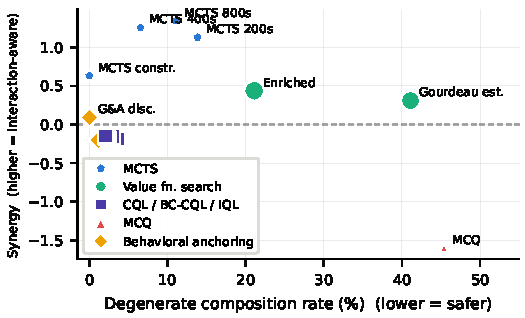
\includegraphics[width=\columnwidth,height=2.12in,keepaspectratio]{fig_safety_context_revision.pdf}
\caption{Safety vs.\ interaction-awareness for each strategy \added{(rich evaluation of Table~\ref{tab:rich}; MCTS points are the leak-free configurations of Table~\ref{tab:mcts})}. Marker size encodes hero diversity; shape and color distinguish method families. Only MCTS configurations reach both low degenerate rate and positive synergy; constraint masking (Section~\ref{sec:constrained}) pins the degenerate rate at zero.}
\label{fig:scatter}
\end{figure}

Fig.~\ref{fig:scatter} summarizes every method on both axes, which require \added{different} solutions. Safety is trivially solved by anchoring to human behavior, and the tighter the anchor the safer (discriminator, then GD, then CQL/BC-CQL), or made exact by structural validity masking (Section~\ref{sec:constrained}); MCQ's non-transferring penalty fails even at safety. Interaction-awareness requires value function search with domain-structured features; no anchored variant achieves it (Table~\ref{tab:rich}).

\subsection{Why Pessimistic Offline RL Collapses}

CQL's pessimism penalizes \textit{all} uncommon state-action pairs, not just bad ones: it cannot distinguish an action that is uncommon because it is structurally bad (a fifth tank) from one whose matchup rarely arises (a niche counter-pick), and it cannot substitute for domain-structured features that encode \textit{why} compositions work.

\subsection{What Transfers Beyond HotS}

\added{Several findings depend on the problem structure rather than on the game:} the safety/interaction-awareness decomposition, since any assembly domain separates structural validity from responsiveness to the opposing set; the anchoring-collapse mechanism, since any terminal-reward assembly problem trained with Monte Carlo returns leaves pessimism only the anchoring pathway; and the validity-masking principle, applicable wherever the invalid region is rule-describable. The interaction metrics also port, requiring only pairwise outcome statistics and a reference behavior policy. The domain content does not transfer: the role taxonomy, specific features, and aggregate heuristics must be rebuilt per domain, and a domain without a large second source of aggregate statistics loses the never-observed-composition signal that targets synthetic data.

\subsection{Practical Implications}

For offline RL practitioners, low degenerate rates may indicate behavioral cloning rather than learned reasoning; reporting action diversity alongside reward detects this collapse.

\added{For anyone building a value function from aggregate outcome statistics and then searching against it: compute the statistics out of fold, check calibration on games outside the statistics, and judge the resulting policy with references the search never saw. In our submitted pipeline the leak cost only half a point of held-out accuracy and was invisible on a leaky test set, yet it produced an apparent feature benefit and an apparent search-depth benefit that independent references do not confirm.}

The collapse is a limitation only when the behavior policy is suboptimal, as here, where anchoring inherits the comfort-driven habits of uncoordinated queue play; where the behavior policy is near-optimal (medical protocols, industrial control), staying near it is the right objective.

Contribution 4's deployment target is a free web tool\footnote{\deployurl} running MCTS in-browser at 50--200 simulations per move.

\subsection{Open Problems}
\label{sec:open}

\textit{The talent stage.} Talent selection at seven in-match levels refines the draft-stage assembly our corpus records. \textit{Patch-driven non-stationarity.} Balance patches shift the reward landscape while preserving combinatorial structure, a natural continual-learning testbed.
\section{Conclusion}

Adversarial team assembly poses a distinctive challenge for learned policies: an exponential state space, data clustered as well as sparse, and a terminal evaluation that must itself be learned. In MOBA drafting, search actively exploits the out-of-distribution optimism of learned value functions to assemble structurally broken teams, and the textbook remedy, algorithmic pessimism, does not repair the failure: with Monte Carlo returns the CQL penalty can only anchor toward the behavior distribution, MCQ collapses to a near-deterministic ten-hero policy, and IQL's near-zero advantages reduce it to behavioral cloning.

The repair that works is layered: domain-structured features give the value function the vocabulary to represent compositional quality; synthetic data supplies safety for shallow greedy deployment; MCTS self-play converts the value function into a policy that is safe and interaction-aware at once; and structural constraint masking removes the residual invalid picks by rule, without anchoring to behavior. \added{The headline evidence is a tournament judged only by references that no agent trained against: MCTS agents win 21 of 22 ordered matchups at 0.60 win probability, well above every anchored method (0.44--0.45), and the mask makes the agent structurally valid by construction at no cost. The evidence also carries a warning. Our first pipeline built its features from statistics containing each game's own outcome; measured against its own value function, deeper search and domain features appeared to add +0.048 and +0.023 win probability, while independent judges measured +0.013 and $-$0.010. Out-of-fold statistics, held-out calibration checks, and independent judges should be standard for any value function learned from aggregate outcomes and then searched.} \removed{The agent sweeps all twenty head-to-head matchups at 0.670 consensus win probability. The enriched features contribute +0.023 WP even under deep search ($p < 0.001$), a gap that data scale narrows but does not close.}

\textit{Limitations.} Single game domain. \added{The independent judges are weaker than an in-corpus model (53.9--56.0\% held-out accuracy against 57.7\%), and each has a blind spot: gN shares our value function's model class; the realized-outcome index cannot judge compositions nobody plays and barely penalizes degenerate teams; the Quick Match judges have never seen a draft and are overconfident on ranked drafts (calibration slope about 0.4). The evidence is their agreement, which is strong for the coarse ordering (search above anchoring) and weaker among the searching agents. The post-snapshot games differ from the corpus in population (late uploads) though not in balance patch. The tournament agents play the MCTS policy's argmax with no search at decision time, and all agents trained against behavioral-cloning opponents, so exploitability against adaptive opponents is untested. The leak-free MCTS runs have five seeds per configuration (the submitted configurations had fifteen); with seed SEs of 0.002--0.004 they resolve differences of about 0.01. The CQL-with-enriched-features rows keep the submission's external features. The fractional-factorial sweep estimates main effects, not all interactions. The submission's ensemble-uncertainty and draft-concentration analyses (supplement) describe the submitted agents; their in-sample validation of favorite hero combinations did not replicate on later games and is withdrawn.} Our validation proceeds in three tiers: statistical validation of the metrics on games outside the statistics (supplement); a blinded expert study in progress, designed with known-outcome anchor drafts because professional judgment is itself tier-limited; and longitudinal forward prediction under real use, pursued through an amateur league (the Nexus Gaming Series) but requiring lead time. An external evaluation on 11{,}034 coordinated-league drafts (supplement) shows modest degradation under distribution shift (\added{57.7\% $\to$ 55.5\% for the leak-free enriched model, and the same drop for the naive model}), concentrated in the least-ladder-like drafts. The composition-quality heuristics depend on role statistics, and interaction-metric magnitudes are snapshot-sensitive. \removed{Two of the four evaluators share no features with the winning agent; the Quick Match judges reproduce the tournament ordering; the agent's hero-pool concentration reflects ground-truth-validated synergy edges.}

\ifanonymous
\section*{AI Disclosure}

Portions of this manuscript's text were drafted and edited with Claude (Anthropic)~\cite{claude}; all experiments, analyses, and claims were designed, verified, and approved by the authors.
\else
\section*{Acknowledgment}

We thank Heroes Profile (heroesprofile.com), whose API supplied both our replay corpus and the aggregate statistics. Heroes of the Storm is a trademark of Blizzard Entertainment. Portions of this manuscript's text were drafted and edited with Claude (Anthropic)~\cite{claude}; all experiments, analyses, and claims were designed, verified, and approved by the authors.
\fi

\section*{Conflicts of Interest}

The authors declare no conflicts of interest.

\begin{thebibliography}{20}

\bibitem{kumar2020conservative}
A.~Kumar, A.~Zhou, G.~Tucker, and S.~Levine, ``Conservative Q-Learning for Offline Reinforcement Learning,'' in \textit{Advances in Neural Information Processing Systems}, vol.~33, pp.~1179--1191, 2020.

\bibitem{levine2020offline}
S.~Levine, A.~Kumar, G.~Tucker, and J.~Fu, ``Offline Reinforcement Learning: Tutorial, Review, and Perspectives on Open Problems,'' \textit{arXiv preprint arXiv:2005.01643}, 2020.

\bibitem{kumar2019stabilizing}
A.~Kumar, J.~Fu, M.~Soh, G.~Tucker, and S.~Levine, ``Stabilizing Off-Policy Q-Learning via Bootstrapping Error Reduction,'' in \textit{Advances in Neural Information Processing Systems}, vol.~32, 2019.

\bibitem{chen2018drafting}
Z.~Chen, Y.~Sun, M.~Seif El-Nasr, and T.-H.~D.~Nguyen, ``The Art of Drafting: A Team-Oriented Hero Recommendation System for Multiplayer Online Battle Arena Games,'' in \textit{Proc. ACM Conf. Recommender Systems (RecSys)}, 2018.

\bibitem{gourdeau2021discriminative}
D.~Gourdeau and L.~Archambault, ``Discriminative Neural Network for Hero Selection in Professional Heroes of the Storm and DOTA 2,'' \textit{IEEE Trans. Games}, vol.~13, no.~4, pp.~380--387, 2021.

\bibitem{lee2022draftrec}
H.~Lee, D.~Hwang, H.~Kim, B.~Lee, and J.~Choo, ``DraftRec: Personalized Draft Recommendation for Winning in Multi-Player Online Battle Arena Games,'' in \textit{Proc. ACM Web Conf. (WWW)}, 2022.

\bibitem{summerville2016draft}
A.~Summerville, M.~Cook, and B.~Steenhuisen, ``Draft-Analysis of the Ancients: Predicting Draft Picks in DotA 2 using Machine Learning,'' in \textit{Proc. AAAI Conf. Artificial Intelligence and Interactive Digital Entertainment (AIIDE)}, vol.~12, no.~2, pp.~100--106, 2016.

\bibitem{chen2021juewudraft}
S.~Chen, M.~Zhu, D.~Ye, W.~Zhang, Q.~Fu, and W.~Yang, ``Which Heroes to Pick? Learning to Draft in MOBA Games with Neural Networks and Tree Search,'' \textit{IEEE Trans. Games}, vol.~13, no.~4, pp.~410--421, 2021.

\bibitem{lyu2022mildly}
J.~Lyu, X.~Ma, X.~Li, and Z.~Lu, ``Mildly Conservative Q-Learning for Offline Reinforcement Learning,'' in \textit{Advances in Neural Information Processing Systems}, vol.~35, 2022.

\bibitem{kostrikov2022iql}
I.~Kostrikov, A.~Nair, and S.~Levine, ``Offline Reinforcement Learning with Implicit Q-Learning,'' in \textit{Proc. Int. Conf. Learning Representations (ICLR)}, 2022.

\bibitem{silver2016mastering}
D.~Silver \textit{et al.}, ``Mastering the Game of Go with Deep Neural Networks and Tree Search,'' \textit{Nature}, vol.~529, no.~7587, pp.~484--489, 2016.

\bibitem{silver2018general}
D.~Silver \textit{et al.}, ``A General Reinforcement Learning Algorithm that Masters Chess, Shogi, and Go through Self-Play,'' \textit{Science}, vol.~362, no.~6419, pp.~1140--1144, 2018.

\bibitem{berner2019dota}
C.~Berner \textit{et al.}, ``Dota 2 with Large Scale Deep Reinforcement Learning,'' \textit{arXiv preprint arXiv:1912.06680}, 2019.

\bibitem{vinyals2019grandmaster}
O.~Vinyals \textit{et al.}, ``Grandmaster Level in StarCraft II using Multi-Agent Reinforcement Learning,'' \textit{Nature}, vol.~575, no.~7782, pp.~350--354, 2019.

\bibitem{fujimoto2021minimalist}
S.~Fujimoto and S.~S.~Gu, ``A Minimalist Approach to Offline Reinforcement Learning,'' in \textit{Advances in Neural Information Processing Systems}, vol.~34, 2021.

\bibitem{gao2023scaling}
L.~Gao, J.~Schulman, and J.~Hilton, ``Scaling Laws for Reward Model Overoptimization,'' in \textit{Proc. Int. Conf. Machine Learning (ICML)}, 2023.

\bibitem{chaslot2008parallel}
G.~M.~J.-B.~Chaslot, M.~H.~M.~Winands, and H.~J.~van~den~Herik, ``Parallel Monte-Carlo Tree Search,'' in \textit{Proc. Int. Conf. Computers and Games}, pp.~60--71, 2008.

\bibitem{wu2019accelerating}
D.~J.~Wu, ``Accelerating Self-Play Learning in Go,'' \textit{arXiv preprint arXiv:1902.10565}, 2019.

\bibitem{kaufman2012leakage}
S.~Kaufman, S.~Rosset, C.~Perlich, and O.~Stitelman, ``Leakage in Data Mining: Formulation, Detection, and Avoidance,'' \textit{ACM Trans. Knowledge Discovery from Data}, vol.~6, no.~4, pp.~15:1--15:21, 2012.

\bibitem{prokhorenkova2018catboost}
L.~Prokhorenkova, G.~Gusev, A.~Vorobev, A.~V.~Dorogush, and A.~Gulin, ``CatBoost: Unbiased Boosting with Categorical Features,'' in \textit{Advances in Neural Information Processing Systems}, vol.~31, 2018.

\bibitem{claude}
Anthropic, ``Claude (Fable 5),'' large language model, 2026.


\end{thebibliography}

\end{document}
